\section{Reducing the Model to One Half}

\Citeauthor{akyuz2022} pointed out in their master thesis, that the model satisfies the property in \Cref{equ:yunus.property.symmetry}.
This means, that there is some symmetry in the model.
In the following, I will reduce the model to only $\theta \mapsto F(\theta) \mod \pi$ and observe what happens in the thin area explored above.
\begin{align}
    F(\theta + \pi) & = F(\theta) + \pi \label{equ:yunus.property.symmetry}
\end{align}

Now, something interesting happens.
\Cref{fig:yunus.pi.2d.full} shows a 2D-scan of the same area that is depicted in \Cref{fig:yunus.2pi.2d.full}.
You can see that the thin areas now have a different color from the bigger areas.
This means that the period of the cycle or cycles in that area now have a higher period.

\begin{figure}
    \centering
    \includegraphics[width=0.6\textwidth]{98_Yunus_modpi/2D_Period/result.png}
    \caption{2D Scan of Halved Original Model}
    \label{fig:yunus.pi.2d.full}
\end{figure}

It is not immediately clear, what is happening.
Looking at the cobwebs helps.
\Cref{fig:yunus.pi.CobwebA2} shows the cycle before the thin area with period 6.
It has period 6 which is exactly one-half the cycle in the full model at the same parameter values for $E_0$ and $\chi_0$, since it is just one-half of the model.
Its symbolic sequence is $\L^3\R^3$.
\todo{relation to other pair of cobwebs, farey adding but no period adding bifurcation, etc.}

\begin{figure}
    \centering
    \begin{subfigure}{0.4\textwidth}
        \centering
        \includegraphics[width=\textwidth]{98_Yunus_modpi/Period6/Cobweb_A2/result.png}
        \caption{Before the thin area begins}
        \label{fig:yunus.pi.CobwebA2}
    \end{subfigure}
    \begin{subfigure}{0.4\textwidth}
        \centering
        \includegraphics[width=\textwidth]{98_Yunus_modpi/Period6/Cobweb_B2/result.png}
        \caption{After the thin area begins}
        \label{fig:yunus.pi.CobwebB2}
    \end{subfigure}
    \begin{subfigure}{0.4\textwidth}
        \centering
        \includegraphics[width=\textwidth]{98_Yunus_modpi/Period6/Cobweb_C2/result.png}
        \caption{the thin area ends}
        \label{fig:yunus.pi.CobwebC2}
    \end{subfigure}
    \begin{subfigure}{0.4\textwidth}
        \centering
        \includegraphics[width=\textwidth]{98_Yunus_modpi/Period6/Cobweb_D2/result.png}
        \caption{After the thin area ends}
        \label{fig:yunus.pi.CobwebD2}
    \end{subfigure}
    \caption{Cobwebs of Halfed Original Model}
\end{figure}
